\documentclass[conference]{IEEEtran}
\IEEEoverridecommandlockouts
\usepackage{cite}
\usepackage{amsmath,amssymb,amsfonts}
\usepackage{algorithmic}
\usepackage{graphicx}
\usepackage{textcomp}
\usepackage{xcolor}
\usepackage{booktabs}
\usepackage{multirow}
\usepackage{url}
\usepackage{tikz}
\usetikzlibrary{positioning,arrows.meta}
\def\BibTeX{{\rm B\kern-.05em{\sc i\kern-.025em b}\kern-.1667em\lower.7ex\hbox{E}\kern-.125emX}}
\begin{document}

\title{Explainable Fake Review Detection for Bangla and Banglish E-Commerce Text}

\author{\IEEEauthorblockN{Syed Abir Hossain, Alim Bin Yeasin, and Shuhrid Abrar}
\IEEEauthorblockA{Department of Computer Science and Engineering\\Bangladesh\\}
}

\maketitle

\begin{abstract}
Fake-review detection in Bangla and Banglish e-commerce text is difficult because labeled data are limited, class distributions are imbalanced, and reviews combine Bangla, English, transliteration, numerals, emojis, and promotional language. This paper presents an explainable, CPU-feasible PySpark pipeline that fuses TF--IDF, Word2Vec, stylometric, promotional, script, and duplicate-structure signals. The final run uses duplicate-aware splitting, class-weighted supervised learning, and confidence- and class-capped pseudo-labeling on an unlabeled BanglishRev pool. On a locked test set of 1,356 BFRD reviews, the selected Random Forest achieves macro-F1 0.9194, fake-review PR-AUC 0.9213, and accuracy 0.9617 using gold labels only. Adding 31,605 capped pseudo-labels decreases macro-F1 to 0.9098 and fake-review PR-AUC to 0.9033. The result supports multi-signal explainable detection while showing that confidence filtering does not remove confirmation bias or domain-shift risk.
\end{abstract}

\begin{IEEEkeywords}
Bangla NLP, fake review detection, opinion spam, code-mixed text, pseudo-labeling, explainable machine learning, PySpark
\end{IEEEkeywords}

\section{Introduction}
Online reviews influence purchase decisions, seller reputation, and platform trust. Artificially generated or coordinated reviews therefore create both economic and social harm. The problem is especially challenging for Bangla and Banglish e-commerce text: the same review can contain Bengali Unicode, Latin transliteration, English product terms, prices, emojis, URLs, informal spelling, and promotional slogans. The project goal is a binary detector that is accurate enough for triage, auditable by analysts, and feasible on CPU-oriented infrastructure.

The completed system treats fake-review detection as an evidence-fusion problem rather than a single text-classification task. It combines lexical evidence, dense sentence-level representations, stylometric and promotional signals, and duplicate structure. It also tests whether an unlabeled BanglishRev pool can improve the classifier through controlled pseudo-labeling. The contribution is therefore an integrated and auditable methodology, not a new classifier. The main contributions are:
\begin{itemize}
\item a Bangla/Banglish multi-signal feature pipeline with explicit privacy-safe text views;
\item duplicate-aware splitting and exact/near-duplicate audits to reduce leakage;
\item confidence-, class-, and volume-capped pseudo-labeling with reduced sample weight;
\item global and local explanations through tree importance, linear coefficients, error analysis, and LIME; and
\item a locked-test comparison showing that a validation gain from semi-supervision did not transfer to the final test set.
\end{itemize}

\section{Data and Problem Formulation}
Let each cleaned review be $x_i$ with binary label $y_i\in\{0,1\}$, where $y_i=0$ denotes fake and $y_i=1$ denotes genuine. The gold source is the Bengali Fake Review Dataset (BFRD); the auxiliary unlabeled source is BanglishRev. The final run scanned 1,746,943 BanglishRev written reviews and retained 322,954 clean rows for feature processing. BFRD contains 9,049 raw rows and 9,034 clean rows after validation and duplicate checks.

\begin{table}[t]
\caption{Final-run data inventory and split protocol.}
\label{tab:data}
\centering\footnotesize
\begin{tabular}{lrrr}
\toprule
Partition & Fake (0) & Genuine (1) & Total\\
\midrule
Gold train & 934 & 5,387 & 6,321\\
Validation & 201 & 1,155 & 1,356\\
Locked test & 201 & 1,155 & 1,356\\
Unlabeled feature pool & -- & -- & 322,954\\
\bottomrule
\end{tabular}
\end{table}

The locked test is evaluated only after model selection. Exact duplicate hashes are audited, and MinHash locality-sensitive hashing (LSH) is used for near-duplicate analysis. Supervised transformations remain train-scoped; the final feature audit records a transductive global fit for unsupervised vocabulary/embedding construction, which is reported explicitly as a validity caveat.

\section{Pipeline and Methodology}
Fig.~\ref{fig:pipeline} gives the complete pipeline. The design separates acquisition, cleaning, leakage control, representation learning, supervised selection, semi-supervised expansion, and explanation.

\begin{figure*}[t]
\centering
\resizebox{\textwidth}{!}{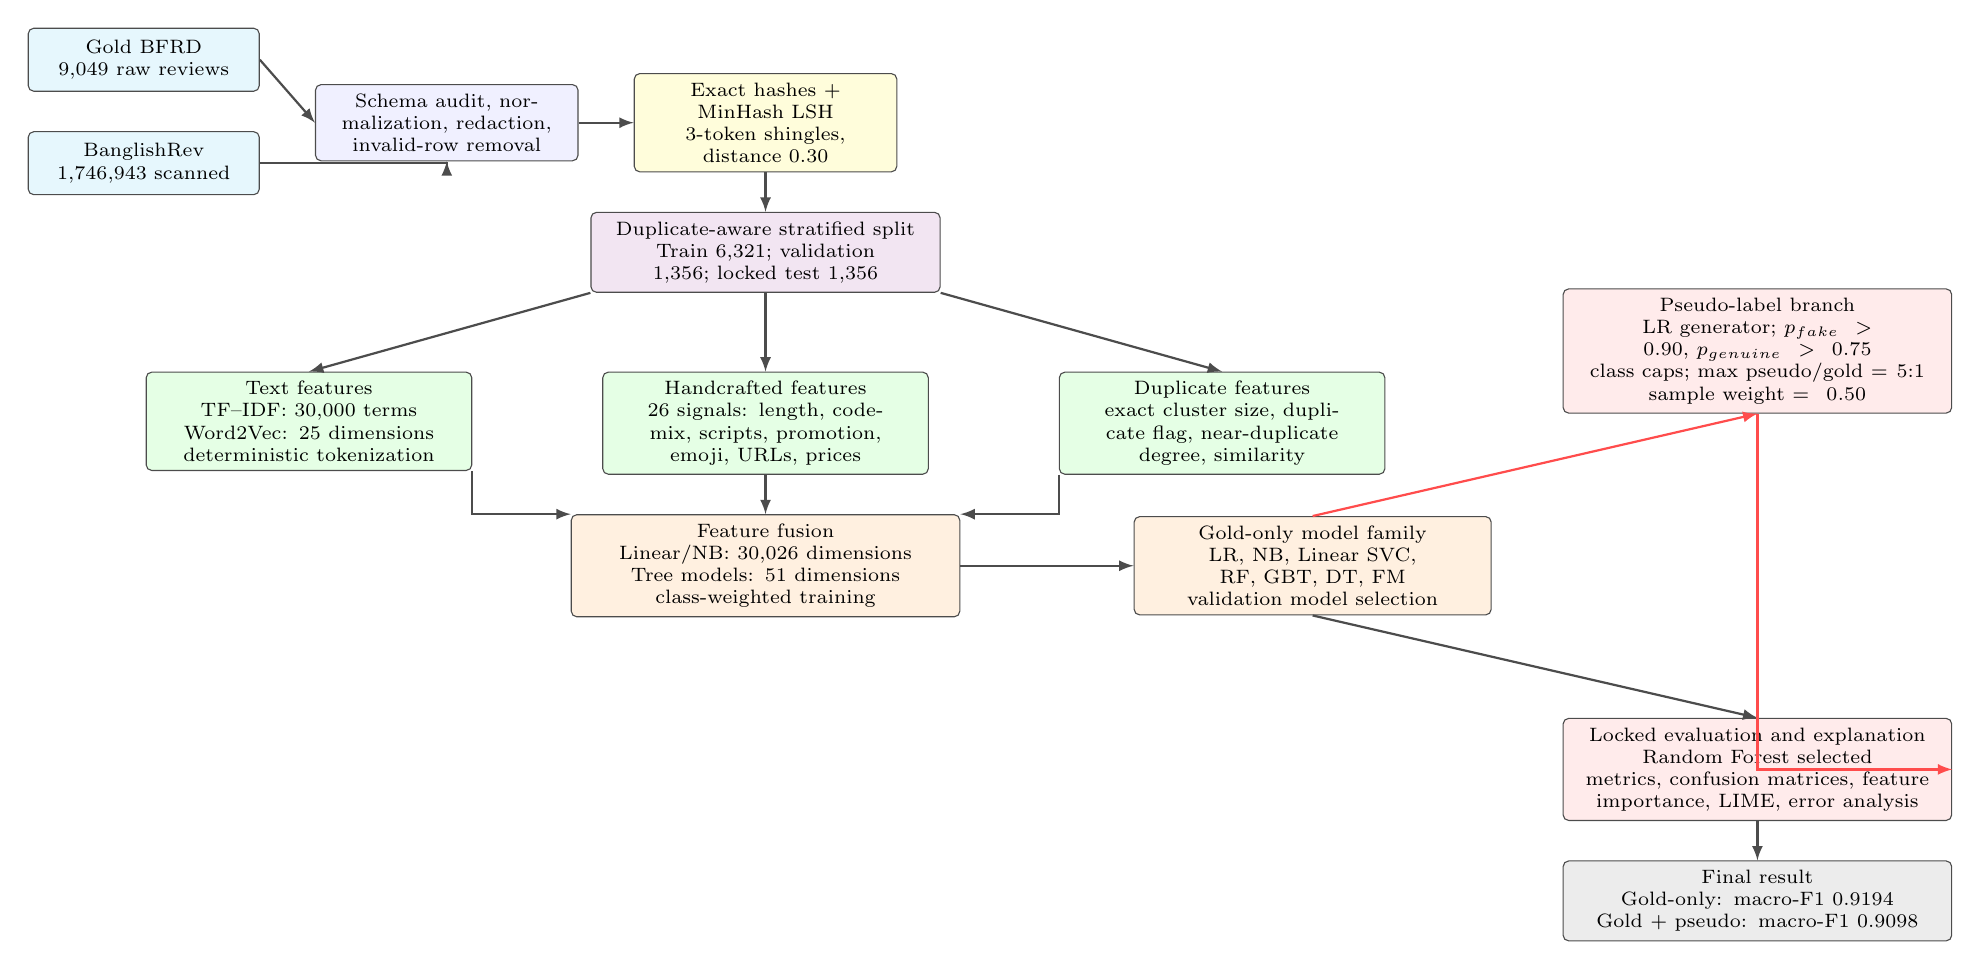
\begin{tikzpicture}[font=\scriptsize, node distance=5mm and 7mm,
  box/.style={draw=black!70, rounded corners=2pt, align=center, minimum height=8mm, text width=27mm, fill=blue!6},
  input/.style={box, fill=cyan!10}, feat/.style={box, fill=green!10}, model/.style={box, fill=orange!12}, outputbox/.style={box, fill=red!8},
  arr/.style={-latex, thick, black!70}]
\node[input] (bfrd) {Gold BFRD\\9,049 raw reviews};
\node[input, below=of bfrd] (bang) {BanglishRev\\1,746,943 scanned};
\node[box, right=of bfrd, yshift=-8mm, text width=31mm] (audit) {Schema audit, normalization, redaction, invalid-row removal};
\draw[arr] (bfrd.east) -- (audit.west); \draw[arr] (bang.east) -| (audit.south);
\node[box, right=of audit, text width=31mm, fill=yellow!14] (dup) {Exact hashes + MinHash LSH\\3-token shingles, distance 0.30};
\draw[arr] (audit.east) -- (dup.west);
\node[box, below=of dup, text width=42mm, fill=violet!10] (split) {Duplicate-aware stratified split\\Train 6,321; validation 1,356; locked test 1,356};
\draw[arr] (dup.south) -- (split.north);

\node[feat, below left=10mm and 15mm of split, text width=39mm] (text) {Text features\\TF--IDF: 30,000 terms\\Word2Vec: 25 dimensions\\deterministic tokenization};
\node[feat, below=10mm of split, text width=39mm] (hand) {Handcrafted features\\26 signals: length, code-mix, scripts, promotion, emoji, URLs, prices};
\node[feat, below right=10mm and 15mm of split, text width=39mm] (graph) {Duplicate features\\exact cluster size, duplicate flag, near-duplicate degree, similarity};
\draw[arr] (split.south west) -- (text.north); \draw[arr] (split.south) -- (hand.north); \draw[arr] (split.south east) -- (graph.north);

\node[model, below=of hand, text width=47mm] (fusion) {Feature fusion\\Linear/NB: 30,026 dimensions\\Tree models: 51 dimensions\\class-weighted training};
\draw[arr] (text.south east) |- (fusion.north west); \draw[arr] (hand.south) -- (fusion.north); \draw[arr] (graph.south west) |- (fusion.north east);
\node[model, right=22mm of fusion, text width=43mm] (train) {Gold-only model family\\LR, NB, Linear SVC, RF, GBT, DT, FM\\validation model selection};
\draw[arr] (fusion.east) -- (train.west);

\node[outputbox, above right=13mm and 9mm of train, text width=47mm] (pseudo) {Pseudo-label branch\\LR generator; $p_{fake}>0.90$, $p_{genuine}>0.75$\\class caps; max pseudo/gold $=5{:}1$\\sample weight $=0.50$};
\draw[arr, red!70] (train.north) -- (pseudo.south);
\node[outputbox, below right=13mm and 9mm of train, text width=47mm] (eval) {Locked evaluation and explanation\\Random Forest selected\\metrics, confusion matrices, feature importance, LIME, error analysis};
\draw[arr] (train.south) -- (eval.north);
\draw[arr, red!70] (pseudo.south) |- (eval.east);
\node[box, below=of eval, text width=47mm, fill=gray!15] (concl) {Final result\\Gold-only: macro-F1 0.9194\\Gold + pseudo: macro-F1 0.9098};
\draw[arr] (eval.south) -- (concl.north);
\end{tikzpicture}
}
\caption{Detailed final-run pipeline and methodology. Red edges denote the controlled pseudo-label branch; the test split remains locked and is never pseudo-labeled.}
\label{fig:pipeline}
\end{figure*}

\subsection{Preprocessing and Privacy-Safe Text Views}
The cleaning stage validates schemas, removes invalid rows, normalizes Unicode and whitespace, and records provenance. Separate text views support privacy-aware analysis: email, phone, URL, price, and mention patterns can be removed from model text, while source identifiers and images are excluded. Tokenization is deterministic and shared by the final evaluation and LIME modules. The feature audit records the following handcrafted variables: character and token length; code-mix ratio; repeated-character ratio; Bengali, Latin, digit, and other-character counts; URL, email, phone, price, hashtag, mention, exclamation, and emoji counts; promotional-keyword hits; exact-duplicate cluster size and flag; near-duplicate degree, similarity, and cluster size; and binary presence flags.

\begin{table}[t]
\caption{Feature groups and model mapping.}
\label{tab:features}
\centering\scriptsize
\begin{tabular}{p{0.22\columnwidth}p{0.27\columnwidth}p{0.36\columnwidth}}
\toprule
Group & Configuration & Main use\\
\midrule
TF--IDF/count & 30,000 vocabulary terms & LR, Linear SVC, NB\\
Word2Vec & 25-dimensional mean vector & RF, GBT, DT, FM\\
Stylometry & lengths, scripts, code-mix, repeated chars & all tree/linear fusion\\
Behavioral & promotion, emoji, URLs, prices, mentions & all tree/linear fusion\\
Duplicate graph & exact and MinHash-derived statistics & audit and ablation\\
\bottomrule
\end{tabular}
\end{table}

\subsection{Lexical and Dense Features}
For a term $t$ and document $d$, term frequency--inverse document frequency is computed as
\begin{equation}
\mathrm{tfidf}(t,d)=\mathrm{tf}(t,d)\log\left(\frac{N+1}{\mathrm{df}(t)+1}\right),
\label{eq:tfidf}
\end{equation}
where $N$ is the number of documents and $\mathrm{df}(t)$ is the document frequency. The final Kaggle-safe run uses a 30,000-term count vocabulary; TF--IDF and non-negative count features are used for linear and Naive Bayes models.

Word2Vec produces a 25-dimensional review representation by averaging token vectors. For review tokens $w_1,\ldots,w_m$ with embeddings $v(w_j)$,
\begin{equation}
z_d=\frac{1}{m}\sum_{j=1}^{m}v(w_j),\quad z_d\in\mathbb{R}^{25}.
\label{eq:w2v}
\end{equation}
The model-ready dimensions are 30,026 for linear/Naive Bayes features and 51 for tree features, including 26 handcrafted variables.

\subsection{Duplicate Structure}
For token-shingle sets $A$ and $B$, the MinHash similarity proxy is based on Jaccard similarity,
\begin{equation}
J(A,B)=\frac{|A\cap B|}{|A\cup B|},
\label{eq:jaccard}
\end{equation}
with a distance threshold of 0.30, three hash tables, 8,192 hash dimensions, and three-token shingles. For each review, graph features summarize local duplicate exposure without directly copying review text.

\subsection{Class-Weighted Models}
The model family includes Logistic Regression (LR), Multinomial Naive Bayes (NB), Linear SVC, Random Forest (RF), Gradient-Boosted Trees (GBT), Decision Tree (DT), and Factorization Machine (FM). For a linear classifier, the probability of a fake review is
\begin{equation}
p_{\mathrm{fake}}(x)=p(y=0\mid x)=\sigma(w^\top x+b)=\frac{1}{1+e^{-(w^\top x+b)}}.
\label{eq:logistic}
\end{equation}
The weighted LR objective is
\begin{equation}
\min_{w,b}\;\frac{\lambda}{2}\lVert w\rVert_2^2+\sum_i \alpha_{y_i}\log\left(1+e^{-y_i(w^\top x_i+b)}\right),
\label{eq:lr_loss}
\end{equation}
where $\alpha_{y_i}$ is the class weight. In the final run, weights are $\alpha_0=3.38383$ for fake reviews and $\alpha_1=0.58669$ for genuine reviews. RF combines trees using
\begin{equation}
\hat{p}_{\mathrm{fake}}(x)=\hat{p}(y=0\mid x)=\frac{1}{T}\sum_{t=1}^{T}h_t(x),
\label{eq:rf}
\end{equation}
where $h_t$ is the probability estimate of tree $t$.

\subsection{Controlled Pseudo-Labeling}
The tuned LR model generates probabilities on the unlabeled pool. A pseudo-label is accepted only when
\begin{equation}
\tilde{y}(x)=\begin{cases}0,&p_0(x)>0.90\\1,&p_1(x)>0.75\\\varnothing,&\text{otherwise},\end{cases}
\label{eq:pseudo}
\end{equation}
then class caps and a maximum pseudo/gold ratio of $5{:}1$ are applied. Accepted pseudo-labels receive sample weight $\omega_p=0.50$, while gold examples retain weight $1$. The primary run accepted 304,667 candidates before capping and 31,605 after capping: 6,321 fake and 25,284 genuine. A sensitivity branch uses a fake threshold of 0.95 and genuine threshold of 0.70.

\subsection{Explainability}
Global evidence is obtained from LR coefficients and tree feature importance. Local evidence is generated with LIME, which fits a local surrogate $g$ around a point $x$ by minimizing
\begin{equation}
\xi(x)=\arg\min_{g\in G}\;L(f,g,\pi_x)+\Omega(g),
\label{eq:lime}
\end{equation}
where $f$ is the RF predictor, $\pi_x$ weights perturbed samples by proximity to $x$, and $\Omega$ controls surrogate complexity. The final audit contains 110 LIME cases.

\section{Experimental Design and Metrics}
The gold split contains 6,321 training, 1,356 validation, and 1,356 locked-test rows. Model selection uses the gold validation split; the final test is scored once for gold-only and gold-plus-pseudo configurations. Accuracy is reported but not used alone because the fake class is imbalanced. For class $c$, precision, recall, and F1 are
\begin{equation}
P_c=\frac{TP_c}{TP_c+FP_c},\quad R_c=\frac{TP_c}{TP_c+FN_c},\quad F1_c=\frac{2P_cR_c}{P_c+R_c}.
\label{eq:metrics}
\end{equation}
Macro-F1 averages $F1_c$ across both classes. Fake PR-AUC summarizes precision--recall behavior for the fake class; ROC-AUC is included as a secondary ranking metric.

\section{Results}
\subsection{Validation Comparison}
Table~\ref{tab:val} reports the gold validation comparison. RF is the best gold-only model by macro-F1 and fake PR-AUC in the final run. Expanded training improves Linear SVC and NB but decreases RF, LR, and GBT, illustrating that pseudo-labeling effects are model-dependent.

\begin{table}[t]
\caption{Gold and expanded validation performance.}
\label{tab:val}
\centering\scriptsize
\begin{tabular}{lrrrr}
\toprule
Model & Gold F1 & Exp. F1 & $\Delta$F1 & Exp. PR-AUC\\
\midrule
RF & 0.9252 & 0.9224 & -0.0028 & 0.9025\\
LR & 0.9094 & 0.9078 & -0.0016 & 0.8843\\
GBT & 0.9074 & 0.9042 & -0.0033 & 0.8984\\
Linear SVC & 0.7758 & 0.8786 & +0.1028 & 0.8590\\
DT & 0.8650 & 0.8690 & +0.0040 & 0.8630\\
NB & 0.7139 & 0.7501 & +0.0362 & 0.5592\\
FM & 0.6673 & 0.6597 & -0.0077 & 0.3609\\
\bottomrule
\end{tabular}
\end{table}

\begin{figure}[t]
\centering
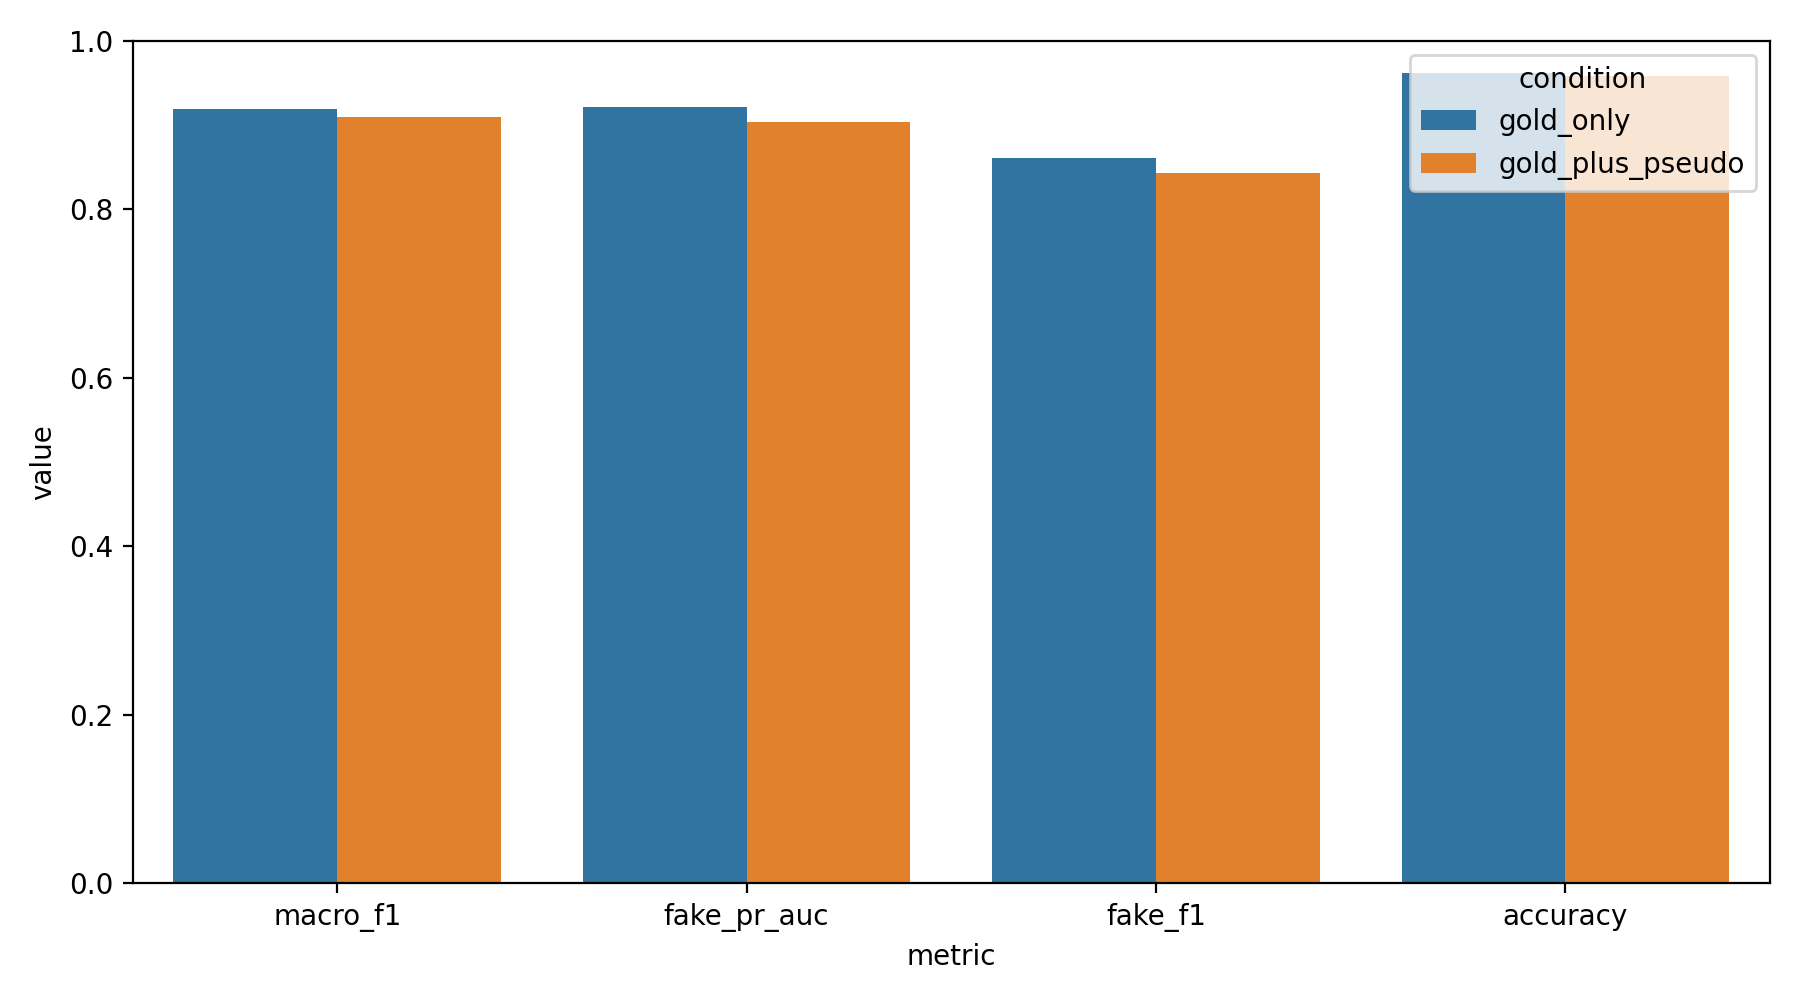
\includegraphics[width=\columnwidth]{report_assets/test_comparison.png}
\caption{Final-run comparison of model and training conditions.}
\label{fig:testcomp}
\end{figure}

\subsection{Locked-Test Evaluation}
Table~\ref{tab:test} uses the machine-readable final evaluation artifact. Gold-only RF is the selected final condition. Its confusion matrix is $[[161,40],[12,1143]]$, where rows are true labels and columns are predictions. Gold-plus-pseudo RF changes this to $[[154,47],[10,1145]]$.

\begin{table}[t]
\caption{Locked-test results for the selected Random Forest.}
\label{tab:test}
\centering\tiny
\begin{tabular}{lrrrrr}
\toprule
Condition & Macro-F1 & Acc. & Fake PR-AUC & Fake F1 & Fake Recall\\
\midrule
Gold only & \textbf{0.9194} & \textbf{0.9617} & \textbf{0.9213} & \textbf{0.8610} & \textbf{0.8010}\\
Gold+pseudo & 0.9098 & 0.9580 & 0.9033 & 0.8438 & 0.7662\\
$\Delta$ & -0.0096 & -0.0037 & -0.0181 & -0.0171 & -0.0348\\
\bottomrule
\end{tabular}
\end{table}

The pseudo-label configuration reduces macro-F1 by 0.0096 and fake PR-AUC by 0.0181. It also reduces fake recall from 0.8010 to 0.7662, while genuine recall increases from 0.9896 to 0.9913. Thus, the capped pseudo-labels make the model slightly more conservative toward the genuine class but less sensitive to fake reviews.

\begin{figure}[t]
\centering
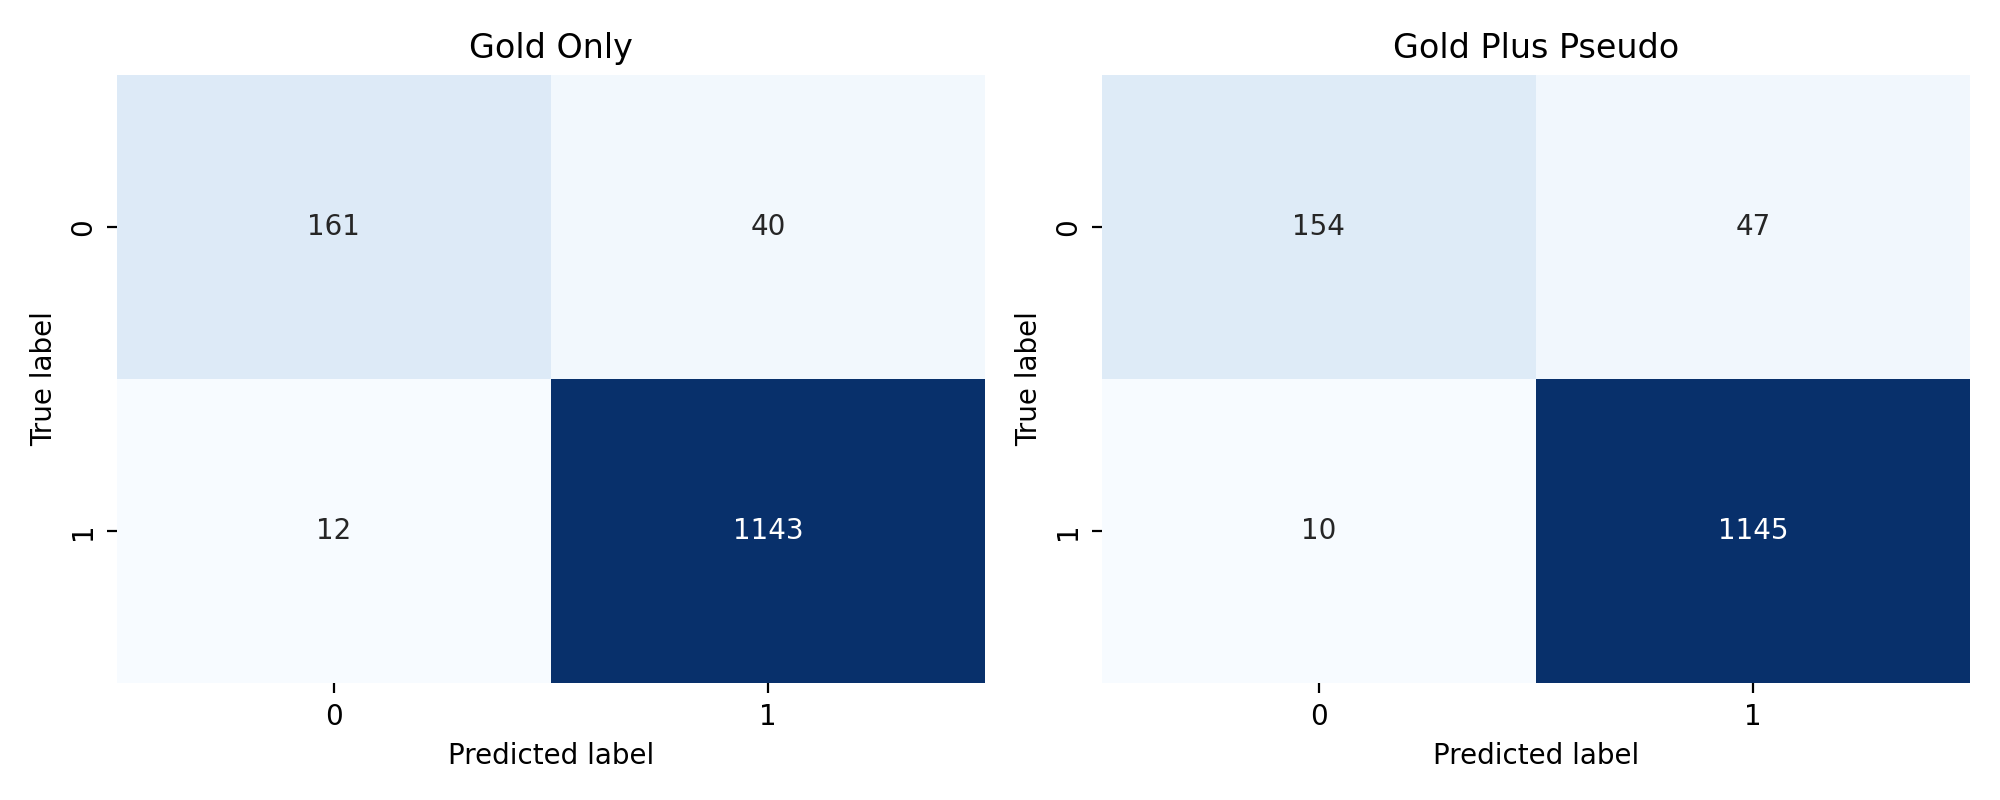
\includegraphics[width=\columnwidth]{report_assets/confusion_matrices.png}
\caption{Confusion matrices for the two locked-test conditions.}
\label{fig:cm}
\end{figure}

\subsection{Ablation and Error Analysis}
Table~\ref{tab:ablation} shows that TF--IDF alone is substantially weaker than the full feature configuration. Removing near-duplicate features changes LR macro-F1 by only +0.0013 in gold validation and leaves expanded performance unchanged, so the current experiment supports their value as an audit signal more strongly than as a dominant predictive component.

\begin{table}[t]
\caption{Feature ablation on validation data.}
\label{tab:ablation}
\centering\scriptsize
\begin{tabular}{llrrr}
\toprule
Cond. & Features & Macro-F1 & PR-AUC & Fake F1\\
\midrule
Gold & Full & 0.9094 & 0.8899 & 0.8446\\
Gold & TF--IDF only & 0.7383 & 0.5919 & 0.5594\\
Gold & No near-dup. & 0.9107 & 0.8901 & 0.8468\\
Expanded & Full & 0.9078 & 0.8843 & 0.8413\\
Expanded & TF--IDF only & 0.7240 & 0.5938 & 0.5551\\
Expanded & No near-dup. & 0.9078 & 0.8843 & 0.8413\\
\bottomrule
\end{tabular}
\end{table}

The final error analysis contains 1,299 correct predictions, 47 false negatives, and 10 false positives. False negatives are shorter on average (450.4 characters and 69.0 tokens) and have higher promotional-hit rates (0.723) than correct cases (674.7 characters, 101.5 tokens, 0.379 promotional hits). False positives are longer (746.3 characters) and always contain at least one promotional hit in the recorded aggregate. This suggests that concise promotional fakes and legitimate promotional language are both difficult cases.

\subsection{Decision-Support Analytics}
The final PySpark SQL notebook was executed against the saved feature and evaluation artifacts and wrote six operational outputs under \texttt{decision\_support\_outputs}. These outputs translate model results into defensible analytics decisions rather than autonomous enforcement decisions.

\begin{table}[t]
\caption{Final decision-support evidence and operational use.}
\label{tab:decisions}
\centering\tiny
\begin{tabular}{p{0.23\columnwidth}p{0.32\columnwidth}p{0.25\columnwidth}}
\toprule
Output & Final evidence & Decision use\\
\midrule
Class balance & 6,321 train; 1,356 validation; 1,356 test. Test has 201 fake and 1,155 genuine. & Use class-aware metrics and weights.\\
Test comparison & Gold-only: macro-F1 0.9194, fake PR-AUC 0.9213, fake recall 0.8010. Expanded: 0.9098, 0.9033, 0.7662. & Keep gold-only as the default condition.\\
Review queue & All 1,356 test predictions ranked by normalized fake-risk score from Random Forest raw class votes. & Prioritize human investigation.\\
Error profile & 1,299 correct, 47 false negatives, and 10 false positives. False negatives average 450.4 characters and 0.723 promotional hits. & Collect more short promotional examples.\\
Duplicate exposure & Four exact-duplicate test rows; mean exact cluster size 1.0029. & Retain duplicate auditing and leakage controls.\\
Drift indicators & Train/validation/test means remain close for length, tokens, code-mix, promotion, emoji, and promo flags. & Continue monitoring; no large split-level shift is indicated.\\
\bottomrule
\end{tabular}
\end{table}

The review queue is for analyst prioritization. It is not proof that a review or seller is fraudulent. The confusion matrices show that pseudo-label expansion misses seven additional fake reviews while reducing two false alarms, so the lower fake-review recall is operationally more important than the small reduction in false positives. The recommended action is human review with explanations, policy evidence, and an appeal path. Drift and duplicate statistics are monitoring signals, not causal evidence.

\begin{figure}[t]
\centering
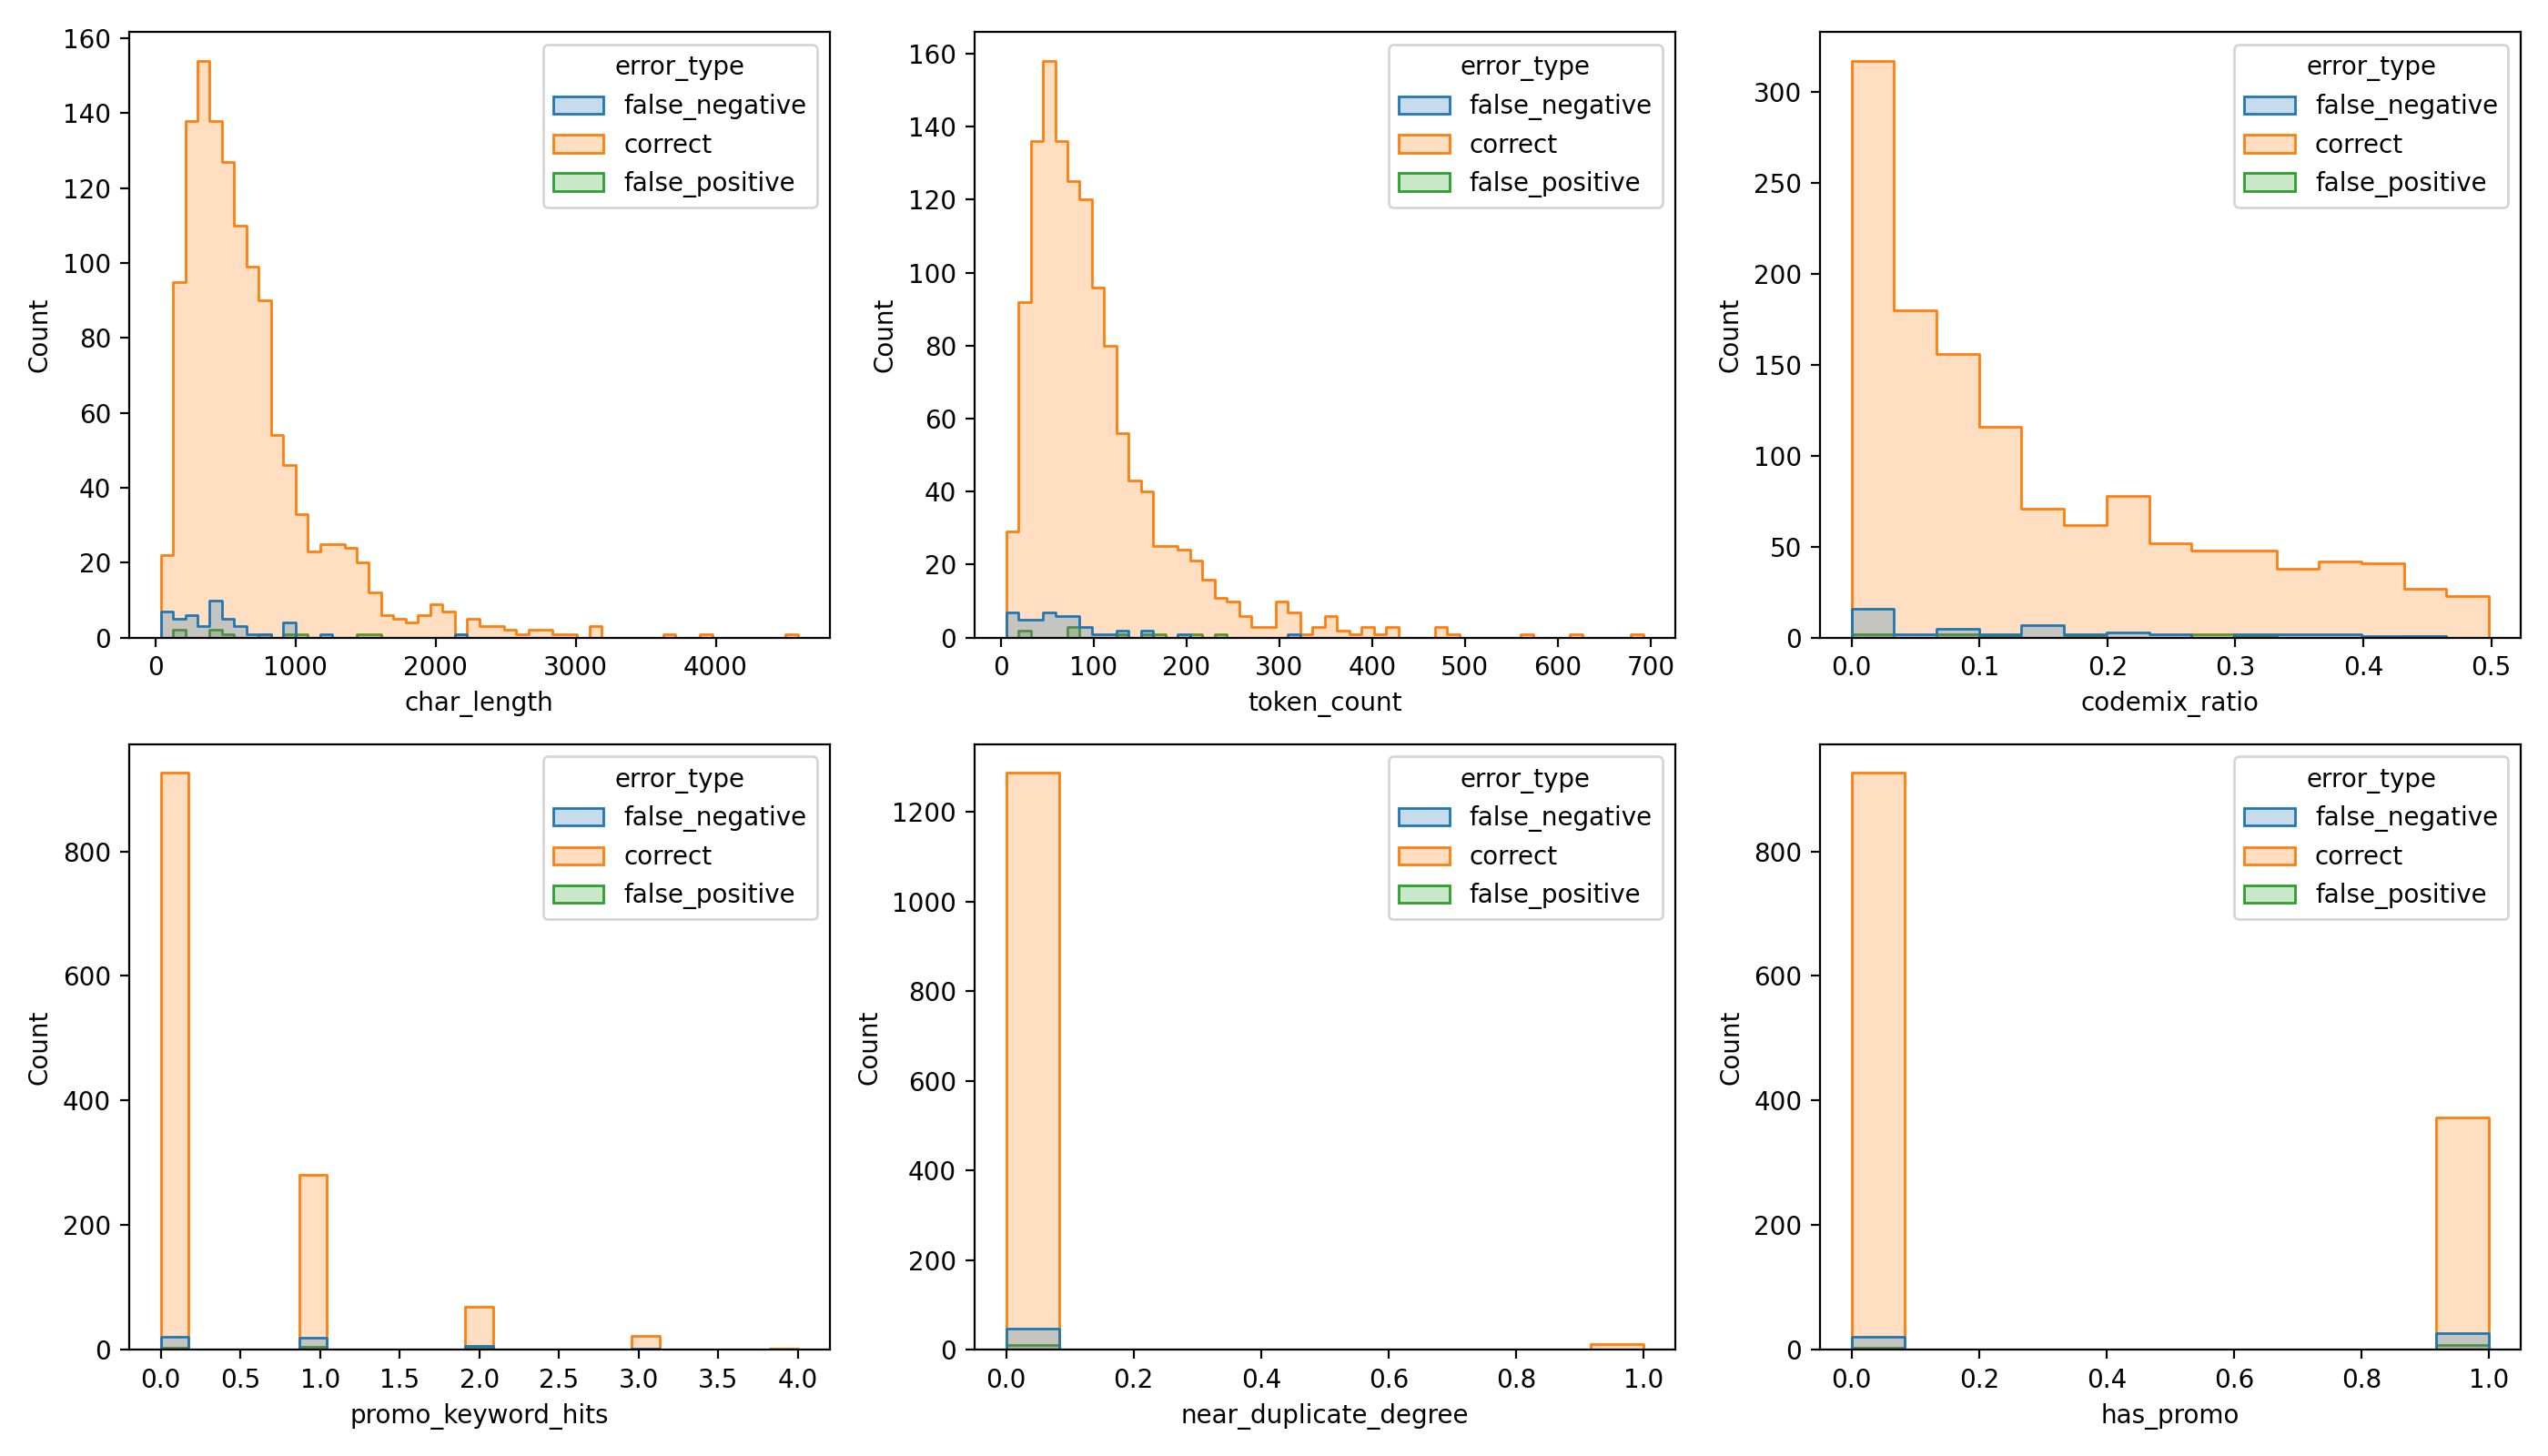
\includegraphics[width=\columnwidth]{report_assets/error_analysis.png}
\caption{Final-run error-analysis visualization.}
\label{fig:error}
\end{figure}

\section{Exploratory Data Analysis and Interpretation}
The project artifacts include class-distribution, length/code-mix, handcrafted-signal, and correlation visualizations. The class distribution motivates macro metrics and class weighting. The length and code-mix plots show why character-level and script-aware signals complement lexical features. The correlation heatmap motivates retaining both raw counts and binary presence features only with care, because correlated signals can inflate tree importance.

\begin{figure*}[t]
\centering
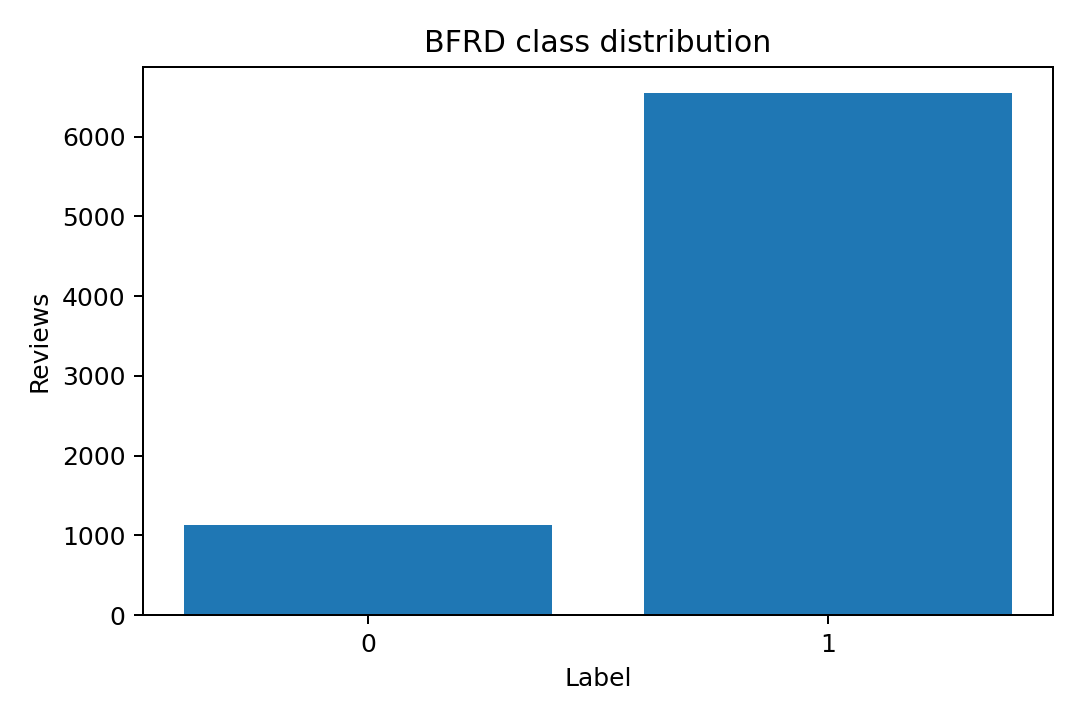
\includegraphics[width=0.31\textwidth]{report_assets/class_distribution.png}\hfill
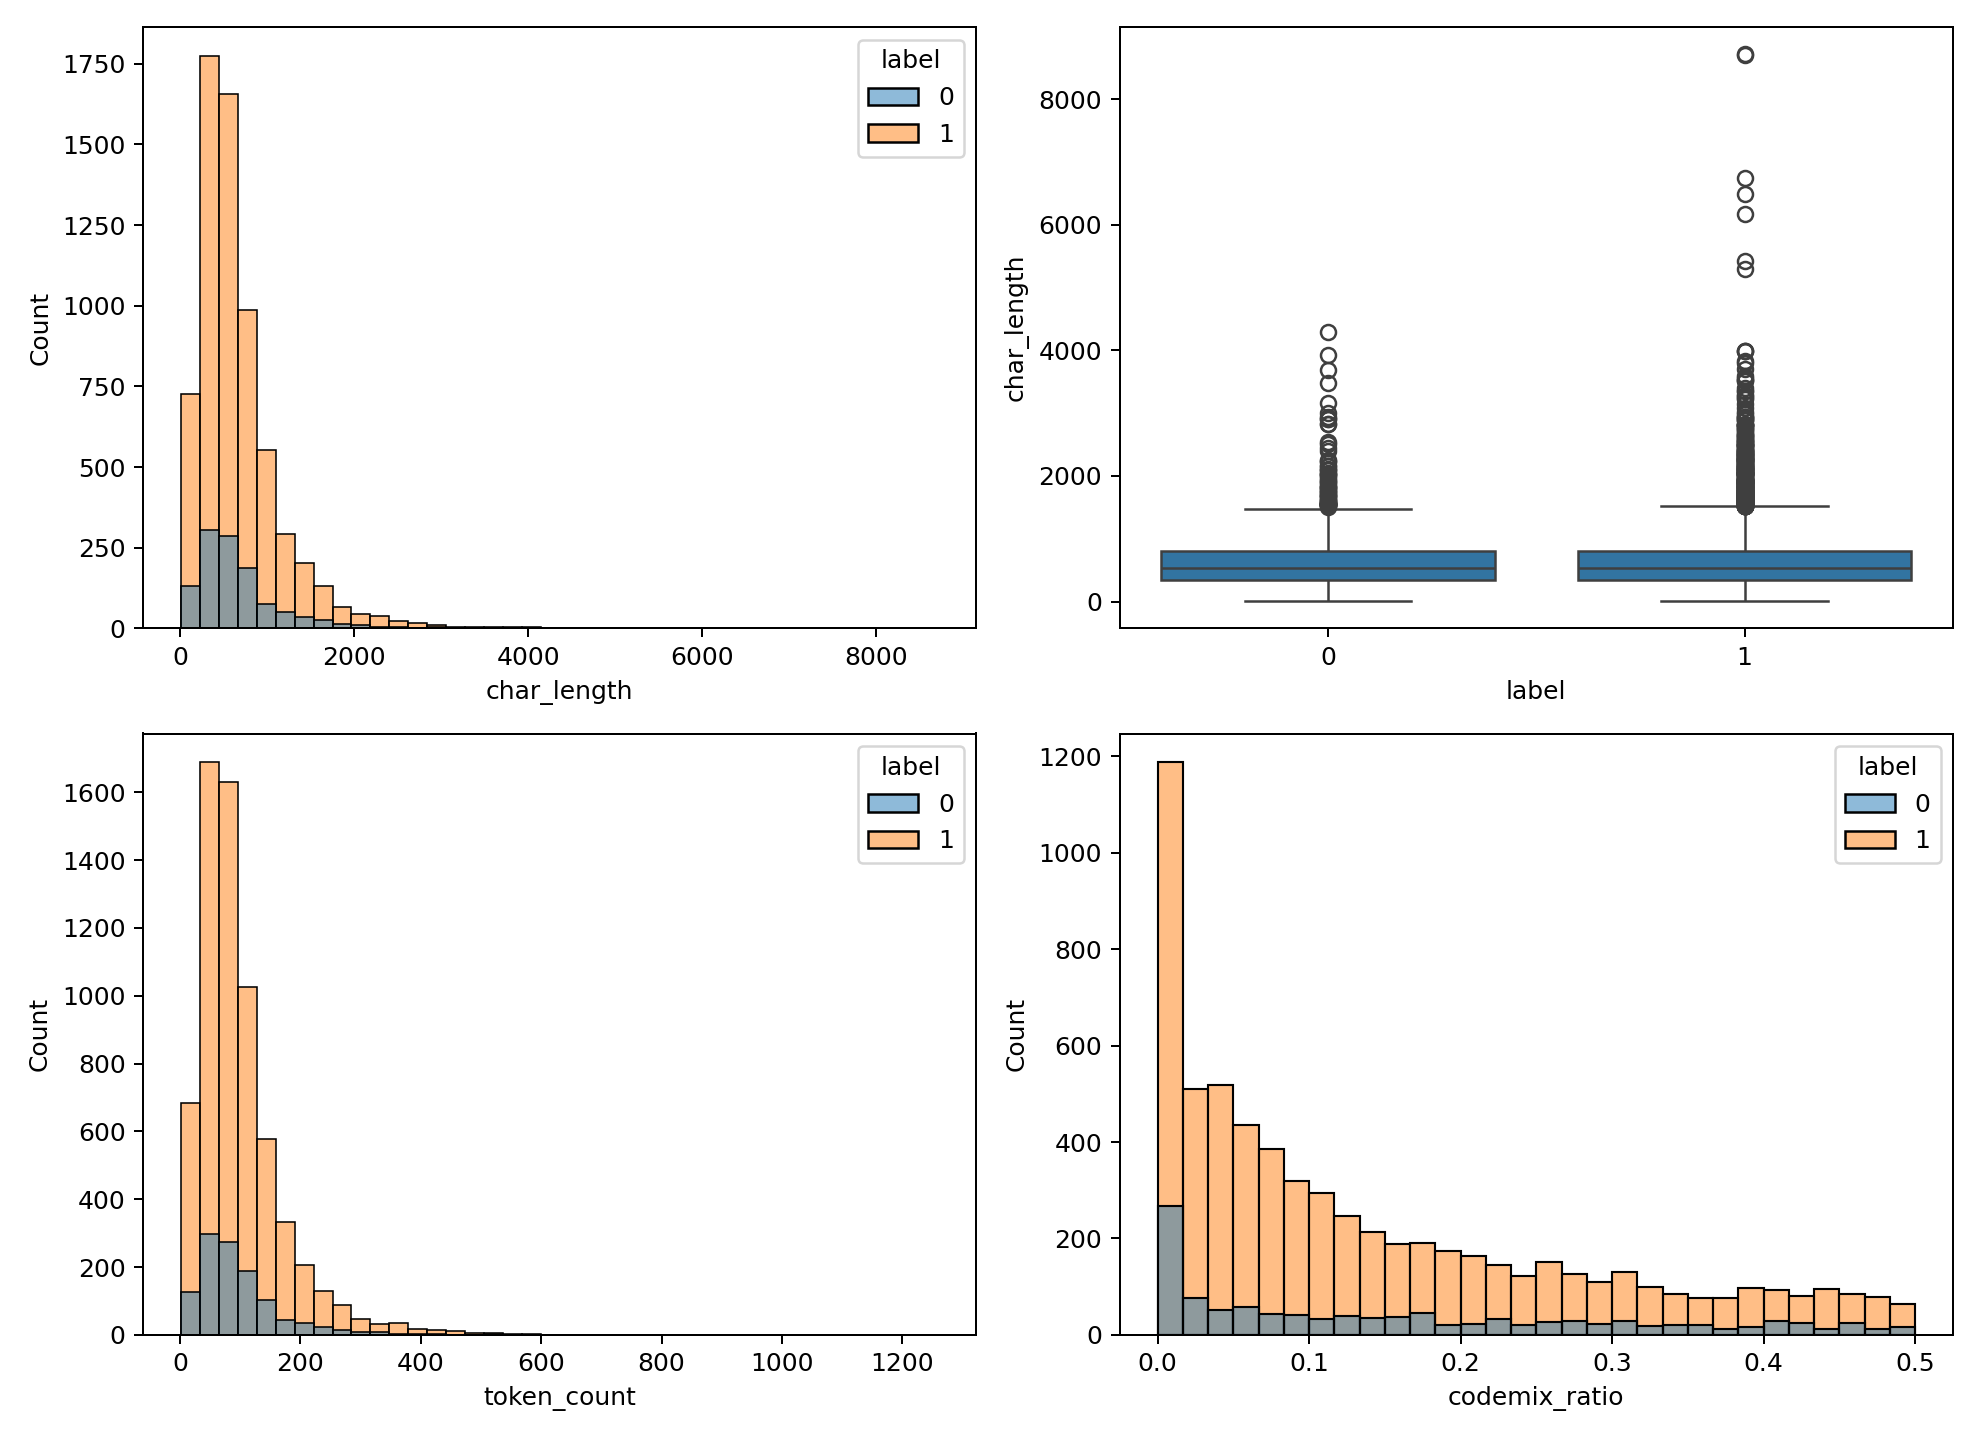
\includegraphics[width=0.31\textwidth]{report_assets/length_token_codemix.png}\hfill
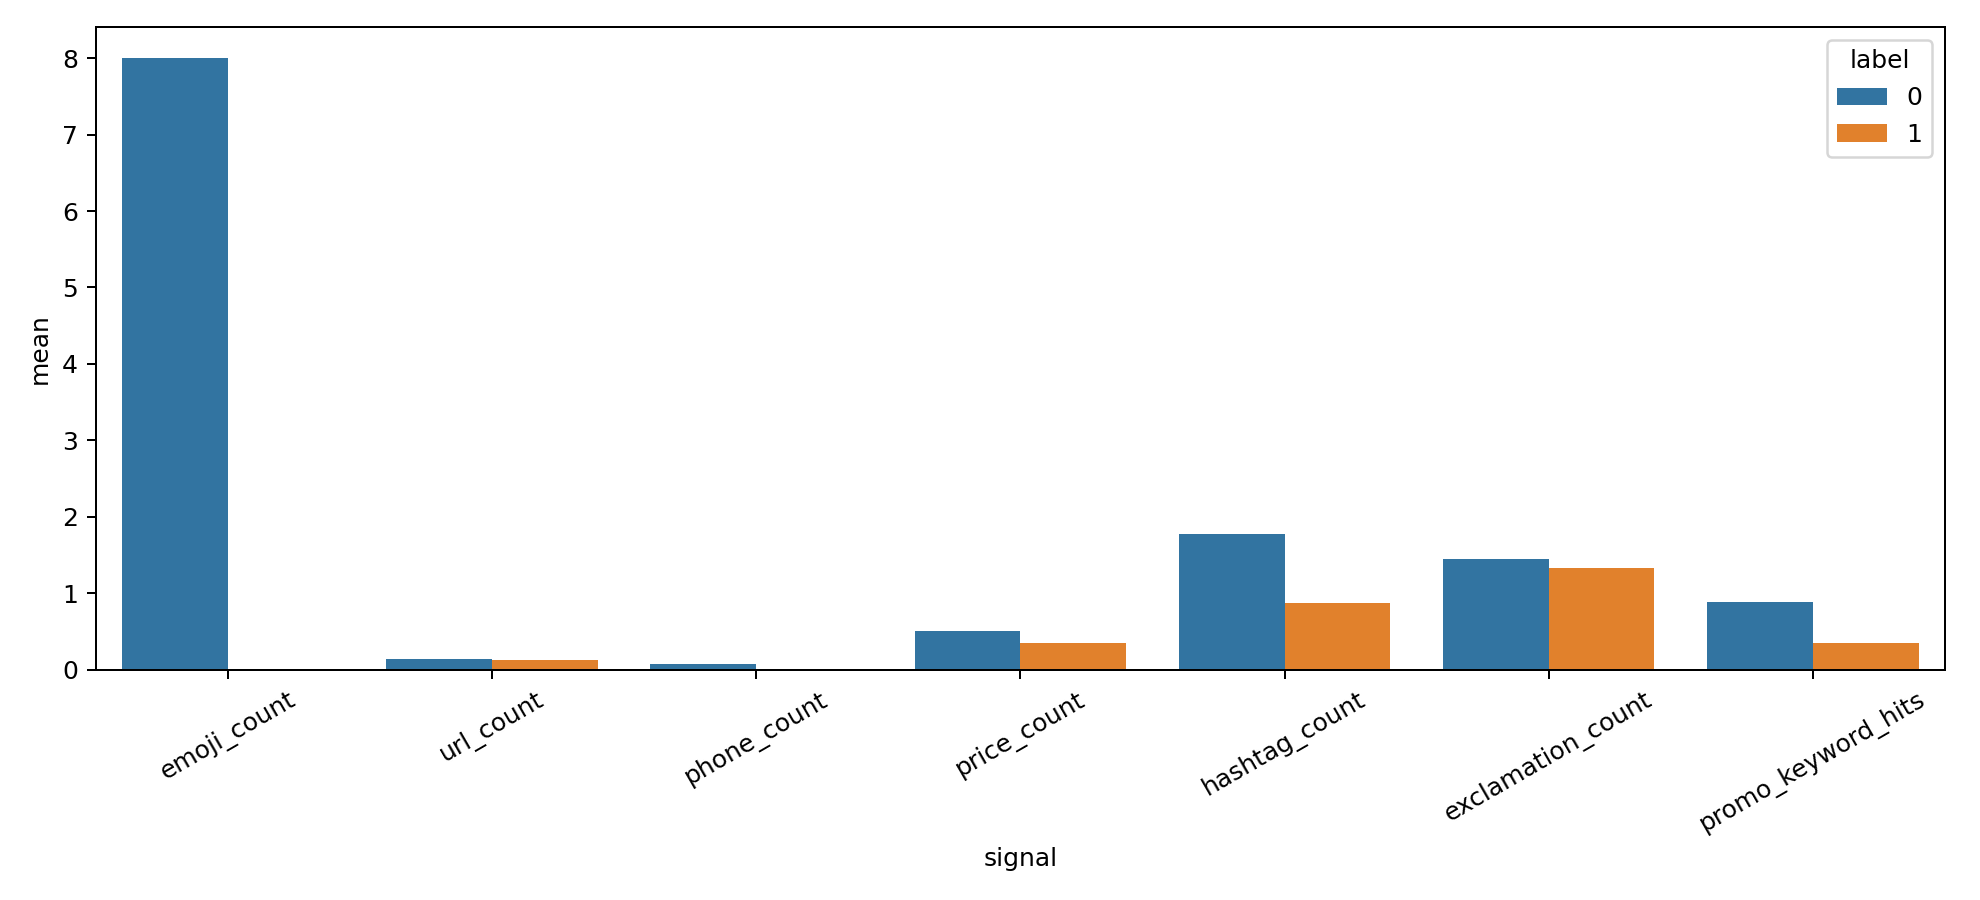
\includegraphics[width=0.31\textwidth]{report_assets/handcrafted_signals.png}
\caption{Selected exploratory visualizations from the final output: class distribution, length/code-mix behavior, and handcrafted signals.}
\label{fig:eda}
\end{figure*}

\begin{figure}[t]
\centering
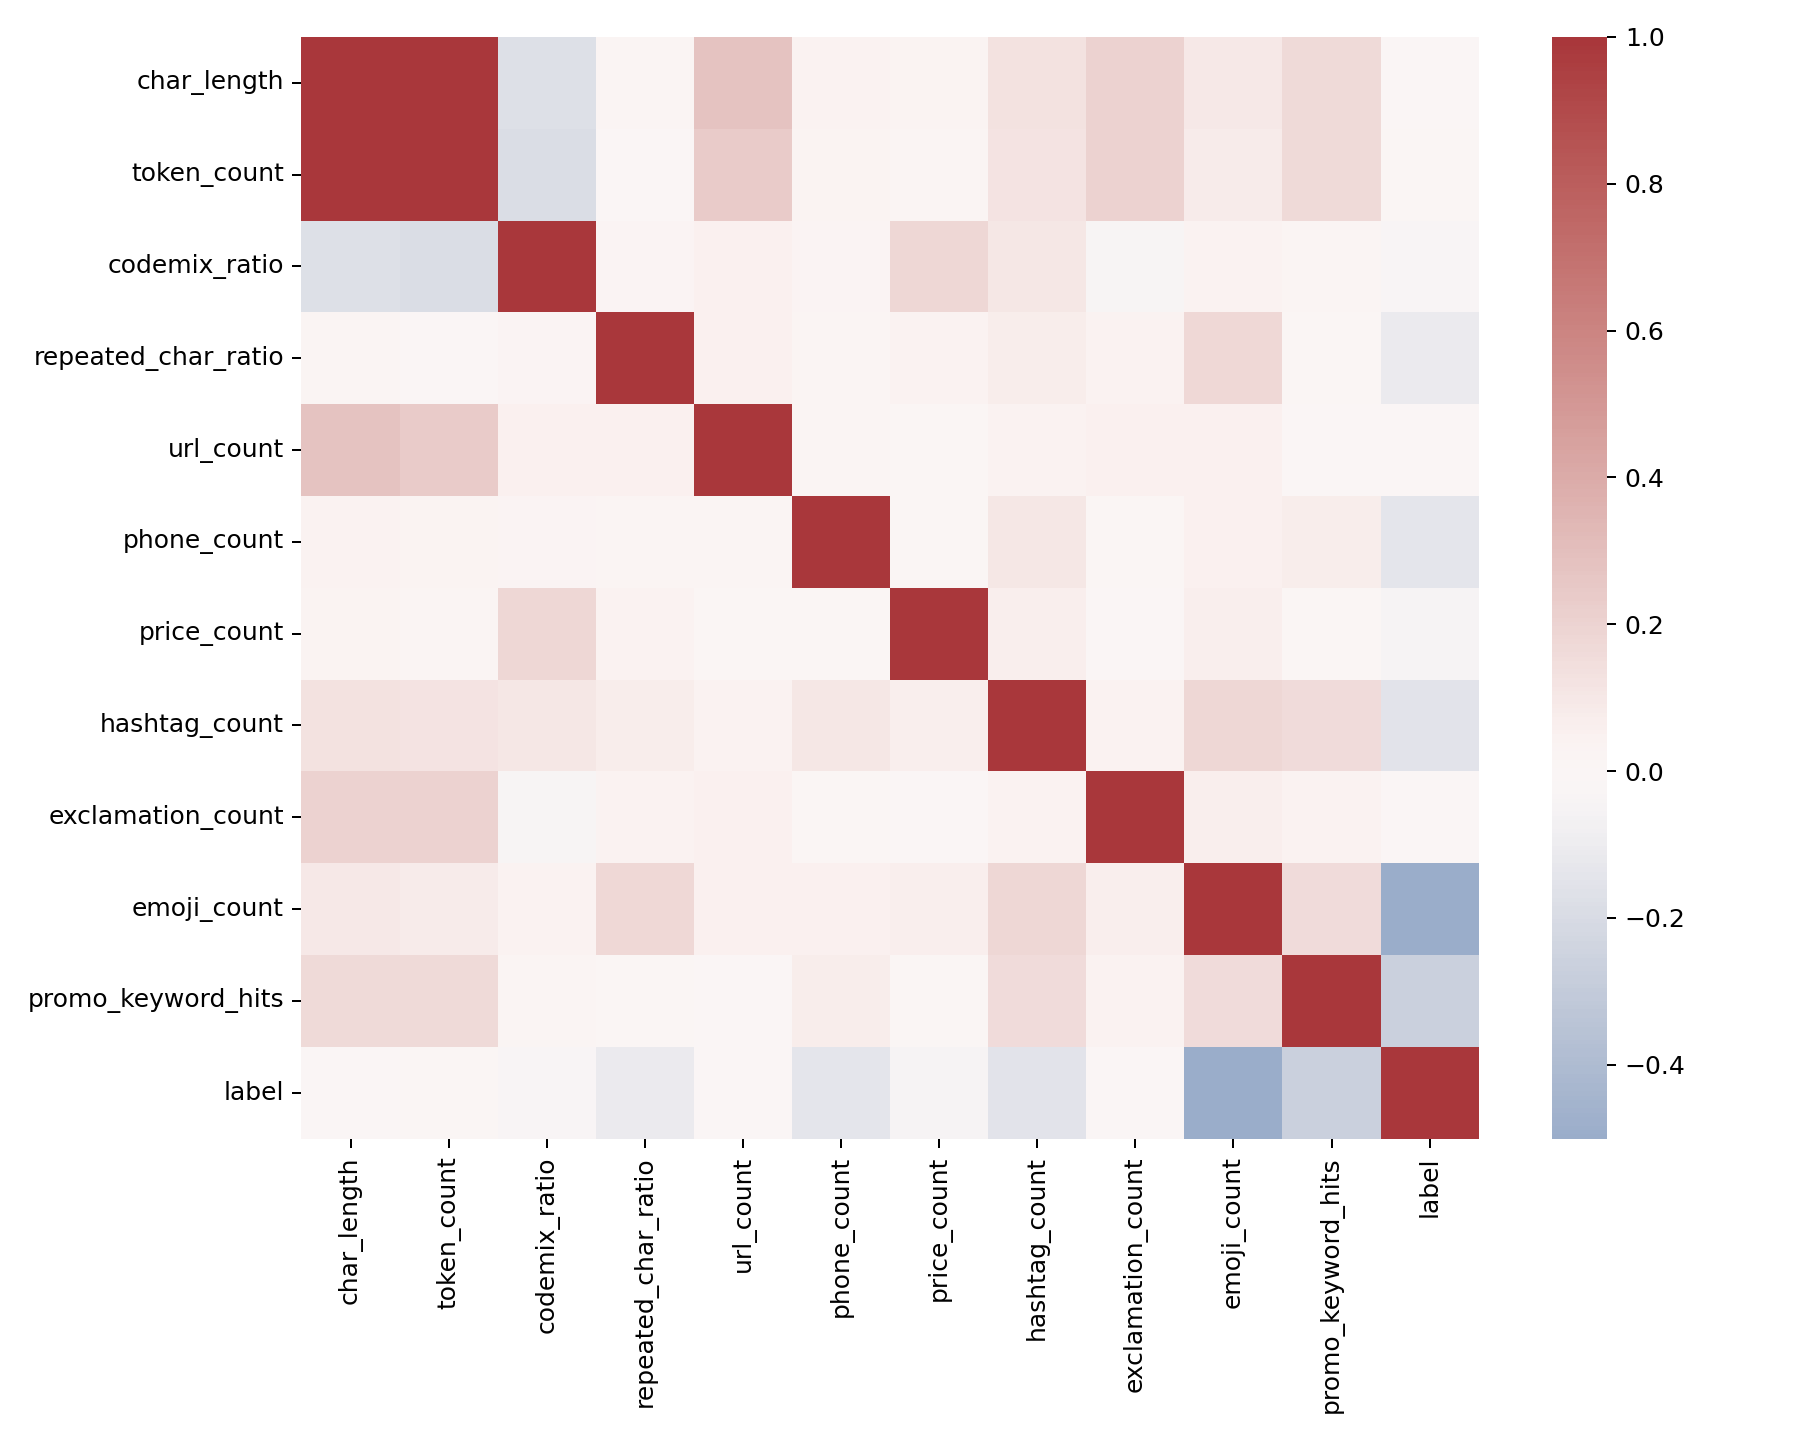
\includegraphics[width=\columnwidth]{report_assets/correlation_heatmap.png}
\caption{Correlation structure among selected handcrafted signals.}
\label{fig:corr}
\end{figure}

Global explanations rank emoji presence/count, latent Word2Vec dimensions, promotional presence, Bengali-character count, and promotional-keyword hits among influential Random Forest inputs. These rankings are associations, not causal rules. LIME explanations provide local evidence for 110 test cases, but their words should be reviewed for privacy before publication and interpreted as surrogate explanations rather than model internals.

\section{Threats to Validity, Ethics, and Limitations}
The detector inherits BFRD annotation and collection bias and has not been externally validated on a second labeled source. BanglishRev is unlabeled and may differ from BFRD, so pseudo-labeling can amplify domain mismatch. The recorded feature audit also reports a global unsupervised fit across gold and unlabeled rows; future releases should make the transductive scope explicit and add a strictly train-fitted comparison. The final run reports point estimates only; bootstrap intervals or repeated splits would strengthen the conclusions.

Deployment should be human-in-the-loop. A prediction should trigger review or ranking, not irreversible seller sanctions, because false positives can damage legitimate businesses and false negatives can leave deceptive content online. Review text may contain personal information; stored artifacts should use hashes or redacted examples, and LIME displays should be screened before release.

\section{Conclusion}
This report documents a reproducible, explainable Bangla/Banglish fake-review detection pipeline built from the final outputs and final run. The selected gold-only Random Forest reaches 0.9194 macro-F1 and 0.9213 fake PR-AUC on the locked test split. The multi-signal feature design is strongly supported by the TF--IDF ablation, while near-duplicate fields are currently more defensible as leakage-control and audit features than as independently validated performance drivers. Most importantly, controlled pseudo-labeling decreases locked-test performance in this run despite useful gains for some validation model families. Future work should add external evaluation, uncertainty intervals, stronger Bangla tokenization, calibration, and human-reviewed pseudo-label audits.

\section*{Acknowledgment}
The authors acknowledge the dataset creators and the open-source Spark and explainability ecosystems used to build the experiment.

\begin{thebibliography}{00}
\bibitem{b1} S. Shahariar et al., ``Bengali fake reviews: A benchmark dataset and detection system,'' \emph{Neurocomputing}, 2024.
\bibitem{b2} M. Shamael et al., ``BanglishRev: A large-scale Bangla-English and code-mixed dataset,'' arXiv:2412.13161, 2024.
\bibitem{b3} N. Jindal and B. Liu, ``Opinion spam and analysis,'' in \emph{Proc. WSDM}, 2008.
\bibitem{b4} M. Ott et al., ``Finding deceptive opinion spam by any stretch of the imagination,'' in \emph{Proc. ACL-HLT}, 2011.
\bibitem{b5} D.-H. Lee, ``Pseudo-label: The simple and efficient semi-supervised learning method for deep neural networks,'' ICML Workshop, 2013.
\bibitem{b6} M. T. Ribeiro, S. Singh, and C. Guestrin, ``Why should I trust you? Explaining the predictions of any classifier,'' in \emph{Proc. KDD}, 2016.
\bibitem{b7} T. Mikolov et al., ``Efficient estimation of word representations in vector space,'' arXiv:1301.3781, 2013.
\end{thebibliography}

\end{document}
